\documentclass[xcolor=dvipsnames]{beamer}
\usetheme{AnnArbor}
\usecolortheme{rose}
\usepackage{ctex}
\usepackage{booktabs}
\usepackage{tabularx}
\usepackage{sistyle}
\usepackage{subfig}
\usefonttheme{professionalfonts}
\setCJKmainfont{黑体} 
\title[微生物土壤运移模型的求解]{\kaishu 微生物土壤运移模型的求解及仿真软件编制\\中期进展报告}
\author{陆秋文}
\institute[北京化工大学]{北京化工大学生命科学与技术学院}
\date{2013年4月9日}
\begin{document}
\AtBeginSection[]
{
    \begin{frame}
        \tableofcontents[currentsection,hideallsubsections]
    \end{frame}
}
\begin{frame}
\titlepage
\end{frame}
\begin{frame}{目录}
\tableofcontents
\end{frame}
\section{研究背景}
	\begin{frame}
	\frametitle{研究背景与意义}
	土壤中微生物的运动是有规律的。在下面这些领域需要对这些规律进行研究:
	\begin{itemize}
	\fangsong
	\item 环境工程领域,对污染的土壤进行治理;
	\item 石油开采,提高开采量;
	\item 放射性物质的携带运输
	\end{itemize}
	\end{frame}
\section{数学模型}
%---------------------------------------------------------------
	\begin{frame}
	\frametitle{假定}
	为了建立数学模型,对过程做如下的假定:
	\begin{itemize}
	\fangsong
	\item 土壤是一个均质体; 
	\item 水流是稳定的; 
	\item 土壤孔隙率是一定的; 
	\item 微生物细胞在液相中均匀悬浮; 
	\end{itemize}\par
	\end{frame}
%--------------------------------------------------------------
	\begin{frame}{微生物在饱和土壤中的迁移方程}
	\begin{block}{\fangsong 迁移方程}
	\begin{equation}\label{qianyif}
	\dfrac{\partial C}{\partial t}=D\dfrac{\partial^2 C}{\partial x^2}-\nu\dfrac{\partial C}{\partial }x-k_{att}\theta C+k_{det}\rho S+\sigma C
	\end{equation}
	\end{block}
	\begin{quote}
	\begin{description}\setlength{\itemsep}{0em}
%	\item[$\theta$]为介质体积含水率,对于饱和土壤,则是介质有效孔隙度;
	\item[$C$]为微生物在水相中的浓度,\SI{}{mg/m^3};
	\item[$S$]为微生物在固体表面可逆吸附的浓度,\SI{}{mg/g};
	\item[$\rho$]为土壤的容重,\SI{}{g/m^3};
	\item[$D$]为水动力弥散系数,\SI{}{m^2/s};
	\item[$v$]为流速,\SI{}{m/s}
	\item[$k_{att}$]为可逆吸附常数,\SI{}{s^{-1}}
	\item[$k_{det}$]为可逆解析常数,\SI{}{s^{-1}}
	\item[$\sigma$]为微生物比生长速率,\SI{}{s^{-1}}
	\end{description}
	\end{quote}
	\end{frame}
%----------------------------------------------------------------
	\begin{frame}{对流扩散反应方程}
	考虑一维上的模型
	\begin{block}{\fangsong 对流扩散反应方程}
	\begin{equation}
	\dfrac{\partial C}{\partial t}= \alpha\dfrac{\partial^2 C}{\partial x^2}-\beta\dfrac{\partial C}{\partial x}-\gamma C + \delta
	\end{equation}
	\end{block}
	\begin{description}\setlength{\itemsep}{0.4em}
	\item[$\dfrac{\partial^2 C}{\partial x^2}$]为扩散项,描述物质的扩散作用;
	\item[$\dfrac{\partial C}{\partial x}$]对流项,描述物质的对流传导作用;
	\item[$C$]为反应项,描述物质在过程中的消耗;
	\item[$\delta$]为生长项,描述物质的产生.
	\end{description}
	\end{frame}
\section{数学模型的参数}
%----------------------------------------------------------------
	\begin{frame}{参数}
	\centering
	\begin{tabularx}{12cm}{XXXXX}
	\toprule
初始浓度 & $v$(\SI{}{cm/min}) & $D$(\SI{}{cm^2/min}) & $\mu$(\SI{}	{min^{-1}}) & $R$\\
	\midrule
$10^6$	&	0.303	&	0.340	&	0.0123	&	1.20 \\
		&	0.608	&	0.607	&	0.0286	&	1.05 \\
		&	0.901	&	0.978	&	0.0362	&	1.02 \\
$10^7$	&	0.303	&	0.316	&	0.0105	&	1.03 \\
		&	0.607	&	0.610	&	0.0183	&	1.00 \\
		&	1.050	&	0.905	&	0.0273	&	1.00 \\
$10^8$	&	0.309	&	0.315	&	0.0106	&	1.00 \\
		&	0.608	&	0.616	&	0.0192	&	1.00 \\
		&	1.060	&	0.917	&	0.0205	&	1.00 \\
	\bottomrule
	\end{tabularx}\end{frame}
%-----------------------------------------------------------
	\begin{frame}
	\begin{center}
	\begin{tabularx}{12cm}{XXXXX}
\toprule
病毒类别 & $v$(cm/s) & $D$(\SI{}{cm^2/h}) & $\mu$(\SI{}{h^{-1}}) & $R$\\
\midrule
IBV		& 3.12	& 0.39	&	0.18	&	1.10	\\
MS2		& 1.60	& 0.10	&	0.09	&	0.98	\\
\bottomrule
\end{tabularx}
	\end{center}\par
	上两表的参数是按照方程
\begin{equation}\label{equ:canshuf}
	R\dfrac{\partial C}{\partial t} = D\dfrac{\partial^2 C}{\partial x^2}-v\dfrac{\partial C}{\partial x}-\mu RC
\end{equation}
所表现的模型测得的,其中$C$的单位为\SI{}{mg/m^3}。
	\end{frame}
%-----------------------------------------------------------
\begin{frame}{参数}
\begin{center}
\begin{tabularx}{12cm}{XXcXX}
\toprule
菌名 & $\alpha$(\SI{}{m^2/s}) & $\beta$(\SI{}{m/s}) & $\gamma$(\SI{}{s^{-1}}) & $\delta$(\SI{}{T^{-1}})\\
\midrule
巨大芽孢杆菌	&	\num{3.66e6}&	\num{0.0006}	&	\num{1.035e-3}	&	\num{7.819e5}	\\
假单胞菌		&	\num{3.66e6}&	\num{0.0006}	&	\num{1.505e-3}	&	\num{1.338e6}	\\
大肠杆菌		&	\num{3.66e6}&	\num{0.0006}	&	\num{5.413e-3}	&	\num{4.547e6}	\\
枯草芽孢杆菌	&	\num{3.66e6}&	\num{0.0006}	&	\num{5.626e-4}	&	\num{2.067e6}	\\
金黄色葡萄球菌	&	\num{3.66e6}&	\num{0.0006}	&	\num{2.037e-3}	&	\num{9.024e5}	\\
微球菌		&	\num{3.66e6}&	\num{0.0006}	&	\num{2.238e-3}	&	\num{1.343e6}	\\
\bottomrule
\end{tabularx}
\end{center}\par
\end{frame}
%----------------------------------------------------------
\begin{frame}
上表的参数是按照方程
\begin{equation}
	\dfrac{\partial C}{\partial t}= \alpha\dfrac{\partial^2 C}{\partial x^2}-\beta\dfrac{\partial C}{\partial x}-\gamma C + \delta
\end{equation}
所表现的模型测得的,其中$C$的单位为\SI{}{mg/m^3}。\par
\end{frame}
%----------------------------------------------------------
\section{问题的数学模型求解}
\begin{frame}{模型}
从问题中得出抽象的数学表达,得到方程~\ref{equ:choux}:
\begin{equation}\label{equ:choux}
	\dfrac{\partial C}{\partial t}= \alpha\dfrac{\partial^2 C}{\partial x^2}-\beta\dfrac{\partial C}{\partial x}-\gamma C + \delta
\end{equation}
这是一个对流扩散反应方程。\par
可以看到$\beta\gg\alpha$,故此方程为一个对流占优的对流扩散反应方程。\par
解这样的一个方程是困难的,我们首先解对流方程,再尝试解对流扩散反应方程。
\end{frame}
\begin{frame}{解对流方程}
忽略掉扩散项,得到方程~\ref{equ:duiliu}
\begin{equation}\label{equ:duiliu}
R\dfrac{\partial C}{\partial t}+v\dfrac{\partial C}{\partial x}= -\mu C + \delta
\end{equation}\par
是一个一阶线性偏微分方程,其定解条件为:
\begin{equation}\label{equ:duiliu_bj}
x=0,t>0,c=c_0
\end{equation}
\begin{equation}
x=\infty,t>0,c=0
\end{equation}
\begin{equation}\label{equ:duiliu_init}
t=0,c=f(x)=0
\end{equation}
这是一个半无界问题。\par
\end{frame}
\begin{frame}
将方程~\ref{equ:duiliu}~作变换,令$a=v/R$、$b=\mu/R$、$D=\delta/R$有
\begin{equation}\label{equ:duiliu_n}
\dfrac{\partial C}{\partial t}+a\dfrac{\partial C}{\partial x}= -b C + D
\end{equation}
令
\begin{equation}\label{equ:duiliu_ys}
\begin{cases}
\xi=x-at \\
\eta=x+at
\end{cases}
\end{equation}
即
\begin{equation}
\begin{cases}
x=\dfrac{1}{2}(\xi+\eta)\\[1.2em]
t=\dfrac{1}{2a}(\eta-\xi)
\end{cases}
\end{equation}
\end{frame}
\begin{frame}
用式~\ref{equ:duiliu_ys}~作映射变换,即
\begin{equation}
\dfrac{\partial C}{\partial \xi}=\dfrac{\partial C}{\partial t}\dfrac{dt}{d\xi}+
								 \dfrac{\partial C}{\partial x}\dfrac{dx}{d\xi}
								=-\dfrac{1}{2a}\dfrac{\partial C}{\partial t}+\dfrac{1}{2}\dfrac{\partial C}{\partial x}						
\end{equation}
\begin{equation}
\dfrac{\partial C}{\partial \eta}=\dfrac{\partial C}{\partial t}\dfrac{dt}{d\eta}+
								 \dfrac{\partial C}{\partial x}\dfrac{dx}{d\eta}
								=\dfrac{1}{2a}\dfrac{\partial C}{\partial t}+
								\dfrac{1}{2}\dfrac{\partial C}{\partial x}		
\end{equation}\par
\end{frame}
\begin{frame}
我们再看方程~\ref{equ:duiliu_n},在变换~\ref{equ:duiliu_ys}~下有
\begin{equation}
2a\dfrac{\partial C}{\partial \eta} = -bC+D
\end{equation}
是比较简单的偏微分方程,它的通解为
\begin{equation}
C=C_1(\xi)e^{-\dfrac{b}{2a}\eta}+\dfrac{D}{b}
\end{equation}
即
\begin{equation}
C(x,t)=C_1(x-at)e^{-\dfrac{b}{2a}(x+at)}+\dfrac{D}{b}
\end{equation}
\end{frame}
\begin{frame}
由初值条件~\ref{equ:duiliu_init},即$\left.C(x,t)\right|_{t=0}=f(x)$,有
\begin{equation}
C_1(x)=e^{\dfrac{b}{2a}}\left(f(x)-\dfrac{D}{b}\right)\quad(x>0)
\end{equation}
由边界条件~\ref{equ:duiliu_bj},即$\left.C(x,t)\right|_{x=0}=c_0$,有
\begin{equation}
C_1(x)=\left(c_0-\dfrac{D}{b}\right)e^{-b\dfrac{b}{2a}x}\quad(x<0)
\end{equation}
整理得
\begin{equation}
C(x,t)=
\begin{cases}
\left(f(x)-\dfrac{D}{b}\right)e^{-bt}+\dfrac{D}{b}  & x-at>0 \\
\left(c_0-\dfrac{D}{b}\right)e^{-\dfrac{b}{a}x}+\dfrac{D}{b}	&x-at<0
\end{cases}
\end{equation}
是对流方程~\ref{equ:duiliu_n}~的解。\par
\end{frame}
\begin{frame}{图象}
\begin{center}
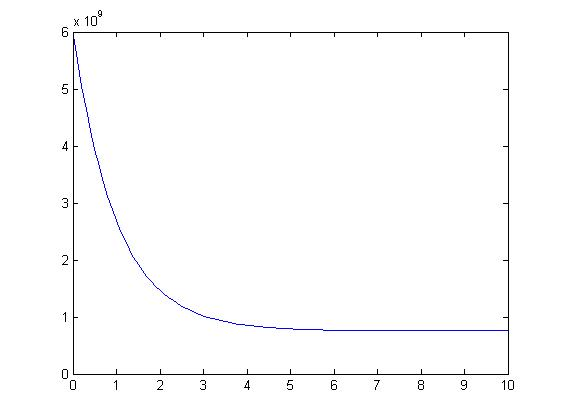
\includegraphics[scale=0.5]{./pic/duiliu.jpg}
\end{center}
\end{frame}
\begin{frame}{解扩散方程}
考虑这样的一个方程,即方程~\ref{equ:kuosan1}
\begin{equation}\label{equ:kuosan1}
	\dfrac{\partial C}{\partial t}-a^2\dfrac{\partial^2 C}{\partial x^2}=0
\end{equation}
它的定解条件为
\begin{equation}
\begin{aligned}\label{equ:kuosan_bianjie}
C(x=0,t)&=0\\
\left.\dfrac{\partial C}{\partial x}\right|_{x=L}&=0
\end{aligned}
\end{equation}
\begin{equation}\label{equ:kuosan_chushi}
\left.C(x,t)\right|_{t=0}=\psi(x)
\end{equation}\par
\end{frame}
\begin{frame}
泛定方程和边界条件都是齐次的,应用分离变数法,其试探解
\begin{equation}
	C(x,t)=X(x)T(t)
\end{equation}
代入方程~\ref{equ:kuosan1}、~\ref{equ:kuosan_bianjie},得
\begin{equation}\label{equ:changX}
	\dfrac{\partial^2 X}{\partial x}+\lambda X=0
\end{equation}
\begin{equation}
	X(0)=0,X'(l)=0
\end{equation}
\begin{equation}
	\dfrac{\partial T}{\partial t}+\lambda a^2 T=0
\end{equation}
\end{frame}
\begin{frame}
考虑$\lambda$为实数的情况,当$\lambda$<0时,方程~\ref{equ:changX}~的解为
\begin{equation}
	X(x)=C_1e^{\sqrt{-\lambda}x}+C_2e^{-\sqrt{-\lambda}x}
\end{equation}
积分常数$C_1$和$C_2$由条件~\ref{equ:kuosan_bianjie}~确定,解得$X(x)=0$,这是没有意义的。\par
同样,当$\lambda$=0时$X(x)=0$,没有意义,我们来看$\lambda$>0时的情况,方程~\ref{equ:changX}~的解为
\begin{equation}
X(x)=C_1\cos \sqrt{\lambda}x+C_2\sin \sqrt{\lambda}x
\end{equation}
\end{frame}
\begin{frame}
积分常数$C_1$和$C_2$由条件~\ref{equ:kuosan_bianjie}~确定,即
\begin{equation}
\begin{gathered}
	C_1 = 0 \\
	C_2\sqrt{\lambda}\cos\sqrt{\lambda}l=0
\end{gathered}
\end{equation}
令$\cos\sqrt{\lambda}l=0$,即$\sqrt{\lambda}l=(k+1/2)\pi(k=0,1,2,\cdots)$,有
\begin{equation}\label{equ:lambda}
\lambda = \dfrac{{\left(k+\dfrac{1}{2}\right)}^2\pi^2}{l^2}=\dfrac{{(2k+1)}^2\pi^2}{4l^2}\quad(k=0,1,2,\cdots)
\end{equation}
给出了本征值,其本征函数为
\begin{equation}
X(x)=C_2\sin\dfrac{(2k+1)\pi}{2l}x\quad(k=0,1,2,\cdots)
\end{equation}\par
\end{frame}
\begin{frame}
我们来看关于$T$的方程,根据式~\ref{equ:lambda},有
\begin{equation}
\dfrac{\partial T}{\partial t} + \dfrac{{\left(k+\dfrac{1}{2}\right)}^2\pi^2}{l^2}a^2T=0
\end{equation}
解为
\begin{equation}
T_k(t)=Ce^{-\dfrac{{\left(k+\dfrac{1}{2}\right)}^2\pi^2 a^2}{l^2}t}\quad(k=0,1,2,\cdots)
\end{equation}\par
这样,$C(x,t)$的解应是
\begin{equation}\label{equ:kuosan_jie1}
	u(x,t)= \sum_{k=0}^{\infty}C_ke^{-\dfrac{{\left(k+\dfrac{1}{2}\right)}^2\pi^2 a^2t}{l^2}}
		    \sin\dfrac{\left(k+\dfrac{1}{2}\right)\pi x}{l}
\end{equation}
\end{frame}
\begin{frame}
将方程~\ref{equ:kuosan1}~代入方程~\ref{equ:kuosan_chushi}~中,有
\begin{equation}
\sum_{k=0}^{\infty} C_k\sin\dfrac{\left(k+\dfrac{1}{2}\right)\pi x}{l} = \psi(x)\quad(0<x<l)
\end{equation}
确定了系数$C_k$.
\end{frame}
\begin{frame}{解对流扩散反应方程}
求解对流扩散反应方程是比较复杂的。现考虑采用线性变换的方法将一阶偏导数项消去,化成单纯的扩散方程再来解。\par
目前,本项工作正在进行。
\end{frame}
\section{有限差分法求解数学模型}
\begin{frame}{简单对流扩散方程的中心差分格式}
考虑一个简单的对流扩散方程
\begin{equation}\label{equ:cf_dkfangc}
	\dfrac{\partial u}{\partial t}+a\dfrac{\partial u}{\partial x}=\nu\dfrac{\partial^2 u}{\partial x^2}
\end{equation}
其中a、$\nu$ 为常数,$\nu>0$,给定初值
\begin{equation}
	u(x,0)=g(x)
\end{equation}
构成了对流扩散方程的初值问题。\par
将方程~\ref{equ:cf_dkfangc}~差分,有
\begin{equation}\label{equ:cf_dkfangct}
	\dfrac{u^{n+1}_j-u^{n}_{j}}{\tau}+a\dfrac{u^{n}_{j+1}-u^n_{j-1}}{2h}=\nu\dfrac{u^n_{j+1}-2u^n_j+u^n_{j-1}}{h^2}
\end{equation}
其截断误差为$O(\tau+h^2)$。\par
\end{frame}
\begin{frame}{稳定性分析}
我们给出用于判断差分格式稳定性的\textbf{von Neumann}~定理,即
\begin{block}{von Neumann定理}
\kaishu
差分格式
\begin{equation}
	u^{n+1}_j=C(x_j,\tau)u^n_j
\end{equation}
稳定的必要条件是当$\tau\leq\tau_0$,$n\tau\leq T$,对所有的k有
\begin{equation}
	\left|\lambda_j(G(\tau,k))\right| \leq 1+M\tau,\quad j=1,2,\cdots,p,
\end{equation}
其中$\left|\lambda_j(G(\tau,k))\right|$表示$G(\tau,k)$的特征值,$M$为常数。
\end{block}
\end{frame}
\begin{frame}
下面来分析差分格式~\ref{equ:cf_dkfangct}~的稳定性,令
\begin{equation}
	\lambda = a\dfrac{\tau}{h},\quad\mu=\nu\dfrac{\tau}{h^2}
\end{equation}
则差分格式~\ref{equ:cf_dkfangct}~改写为
\begin{equation}\label{equ:cf_dkmmm}
u^{n+1}_j=u^n_j-\frac{1}{2}\lambda(u^n_{j+1}-u^n_{j-1})+\mu(u^n_{j+1}-2u^n_j+u^n_{j-1})
\end{equation}\par
式~\ref{equ:cf_dkmmm}~的增长因子为
\begin{equation}
	G(\tau,k)=1-2\mu(1-\cos kh)-i\lambda\sin kh
\end{equation}
模的平方为
\begin{equation}
\begin{aligned}
	|G(\tau,k)|^2 &= 1-(1-\cos kh)[4\mu-4\mu^2(1-\cos kh)-\lambda^2(1+\cos kh)]
\end{aligned}				  
\end{equation}
\end{frame}
\begin{frame}
差分格式稳定的充分条件为
\begin{equation}
4\mu-4\mu^2(1-\cos kh)-\lambda^2(1+\cos kh) \geq 0
\end{equation}
即
\begin{equation}
(2\lambda^2-8\mu^2)\dfrac{1-\cos kh}{2}+4\mu-2\lambda^2 \geq 0
\end{equation}
注意到$\dfrac{1}{2}(1-\cos kh)\in[0,1]$,上式应满足
\begin{equation}
(2\lambda^2-8\mu^2)+4\mu-2\lambda^2 \geq 0,\quad 4\mu-2\lambda^2 \geq 0
\end{equation}
由此得到差分格式~\ref{equ:cf_dkfangct}~的稳定性限制为
\begin{equation}
\tau \leq \dfrac{2\nu}{a^2}
\end{equation}
\begin{equation}
\nu\dfrac{\tau}{h^2}=\dfrac{1}{2}
\end{equation}\par
\end{frame}
\section{模型仿真的结果}
\begin{frame}{巨大芽孢杆菌}
\begin{figure}[h]
\subfloat[$t=10$]{\centering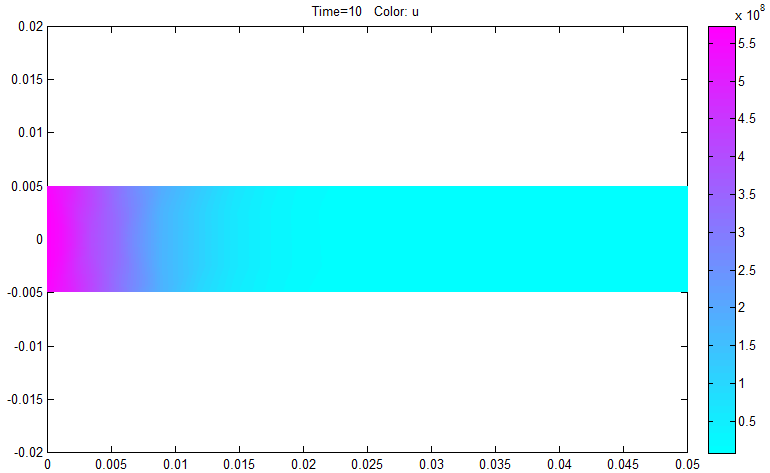
\includegraphics[scale=0.2]{./pic/01.png}}
\subfloat[$t=100$]{\centering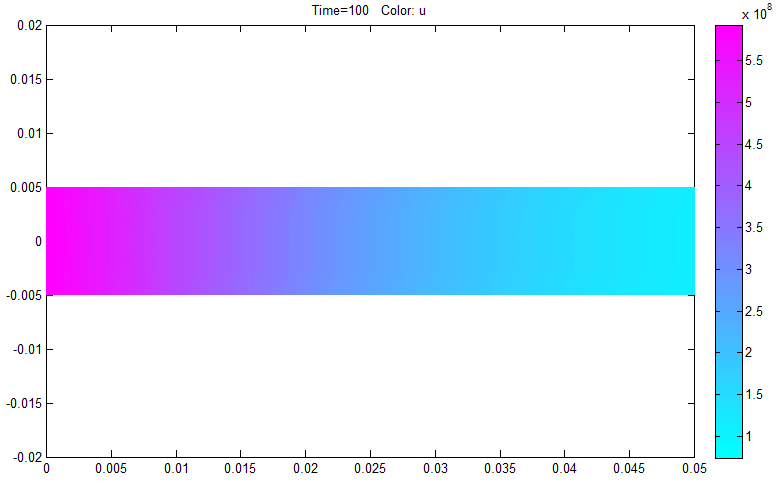
\includegraphics[scale=0.2]{./pic/01-100.png}}
\subfloat[$t=600$]{\centering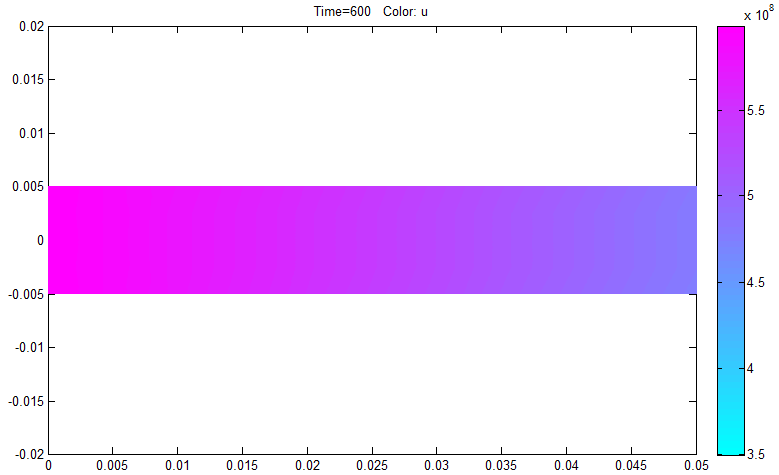
\includegraphics[scale=0.2]{./pic/01-600.png}}
%\caption{巨大芽孢杆菌的仿真结果}\label{pic:1}
\end{figure}
%\begin{figure}
%\setlength{\abovecaptionskip}{0pt}
%\setlength{\belowcaptionskip}{0pt}
%\subfloat[巨大芽孢杆菌]{\centering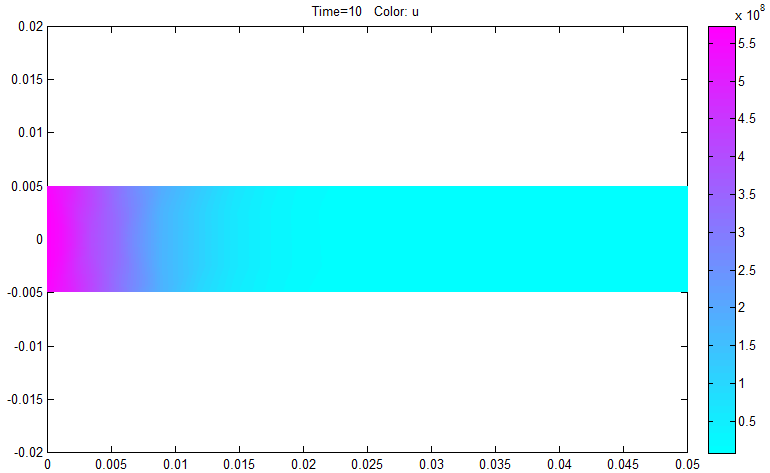
\includegraphics[scale=0.2]{./pic/01.png}}
%\subfloat[假单胞菌]{\centering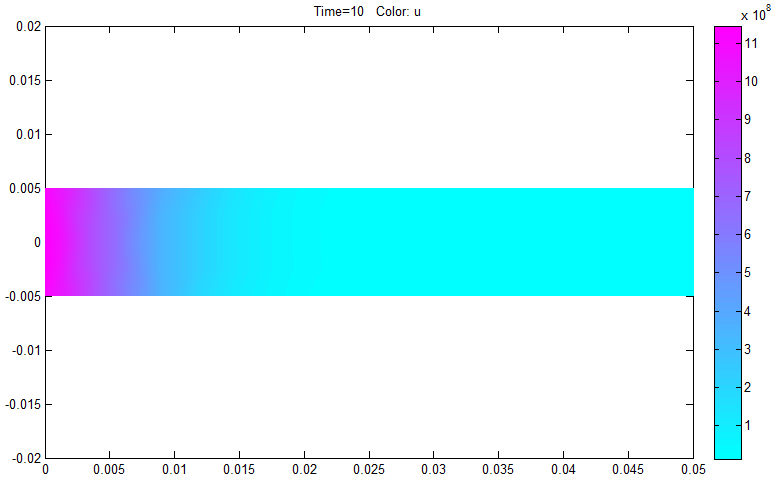
\includegraphics[scale=0.2]{./pic/02.png}}
%\subfloat[大肠杆菌]{\centering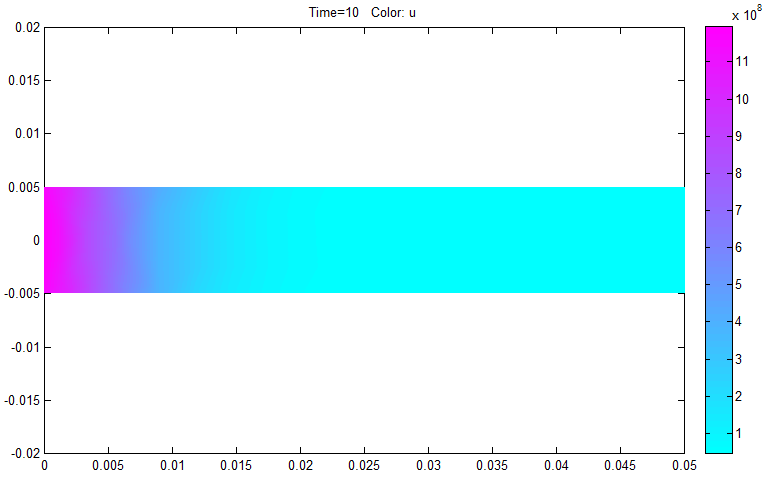
\includegraphics[scale=0.2]{./pic/03.png}}
%
%\end{figure}
\end{frame}
\begin{frame}{假单胞菌}
\begin{figure}[h]
\subfloat[$t=10$]{\centering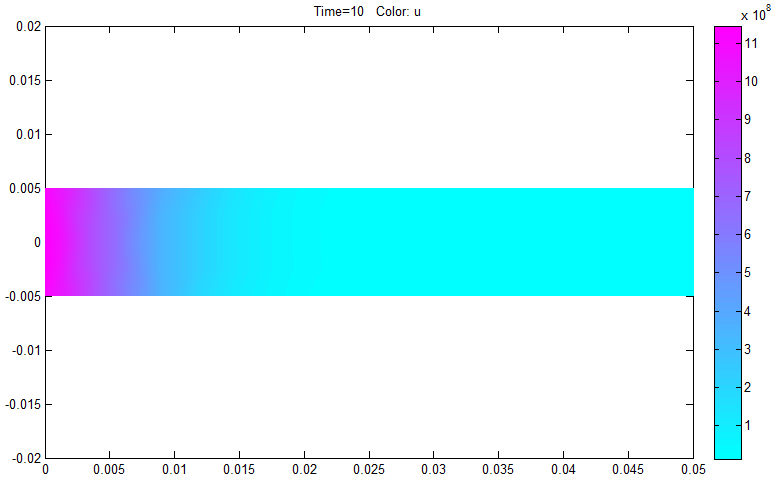
\includegraphics[scale=0.2]{./pic/02.png}}
\subfloat[$t=100$]{\centering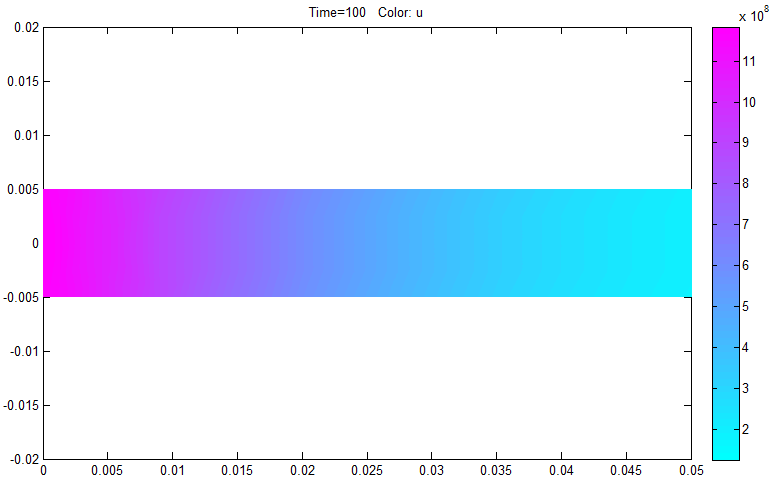
\includegraphics[scale=0.2]{./pic/02-100.png}}
\subfloat[$t=600$]{\centering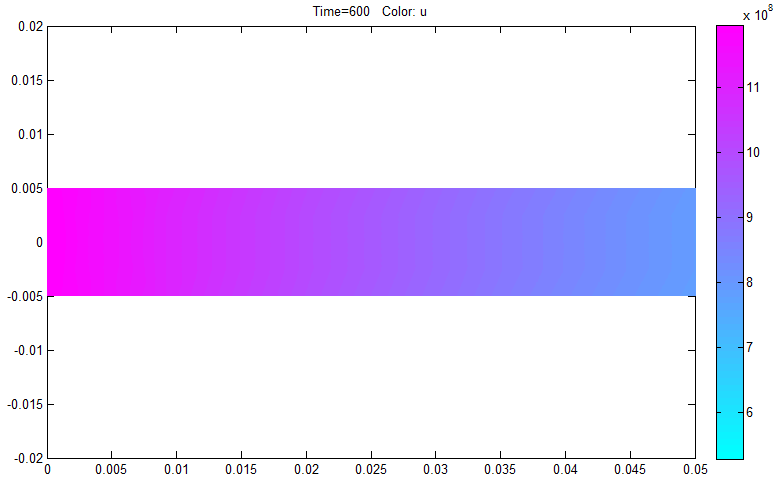
\includegraphics[scale=0.2]{./pic/02-600.png}}
%\caption{巨大芽孢杆菌的仿真结果}\label{pic:1}
\end{figure}
\end{frame}
\begin{frame}{大肠杆菌}
\begin{figure}[h]
\subfloat[$t=10$]{\centering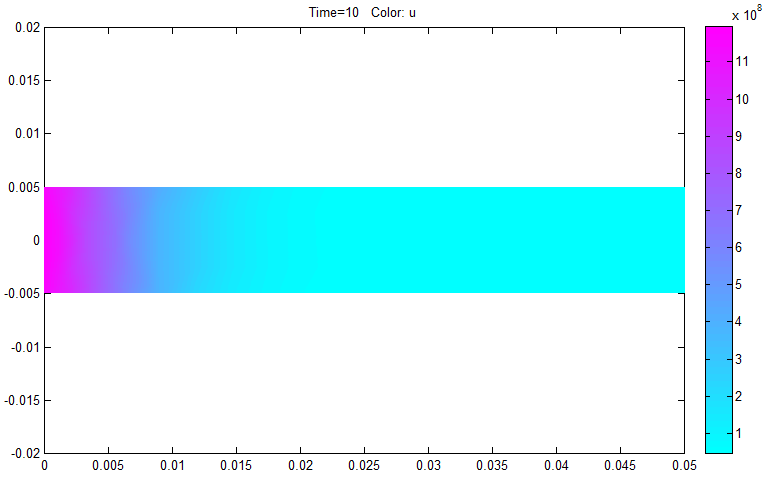
\includegraphics[scale=0.2]{./pic/03.png}}
\subfloat[$t=100$]{\centering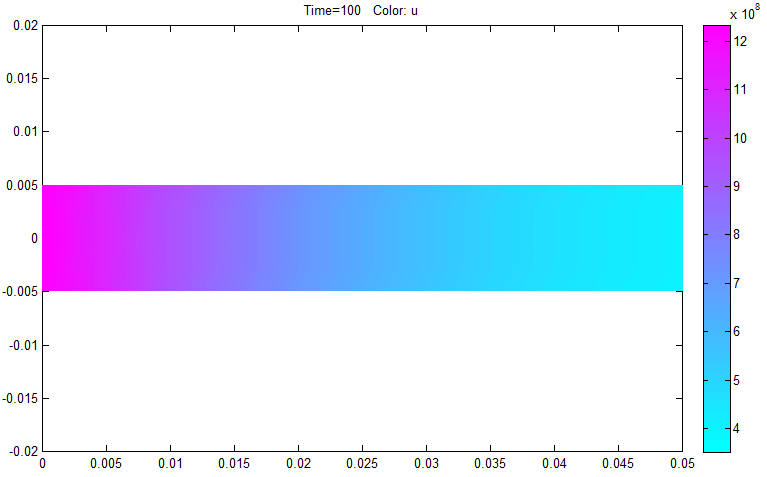
\includegraphics[scale=0.2]{./pic/03-100.png}}
\subfloat[$t=600$]{\centering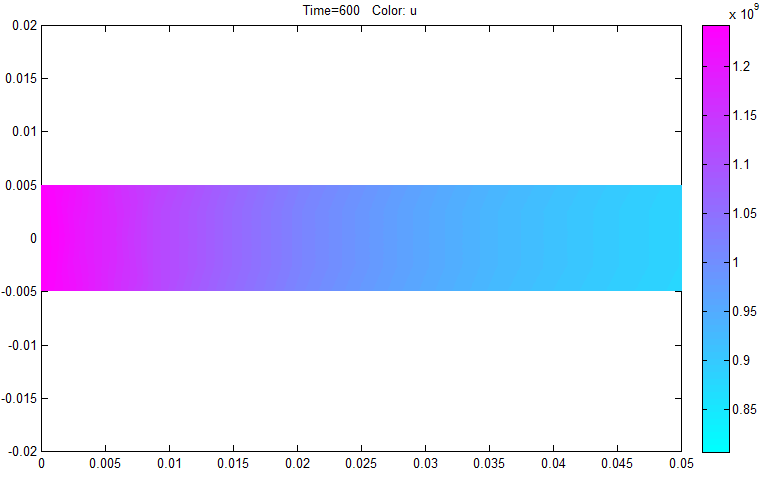
\includegraphics[scale=0.2]{./pic/03-600.png}}
%\caption{巨大芽孢杆菌的仿真结果}\label{pic:1}
\end{figure}
\end{frame}
\begin{frame}{枯草芽孢杆菌}
\begin{figure}[h]
\subfloat[$t=10$]{\centering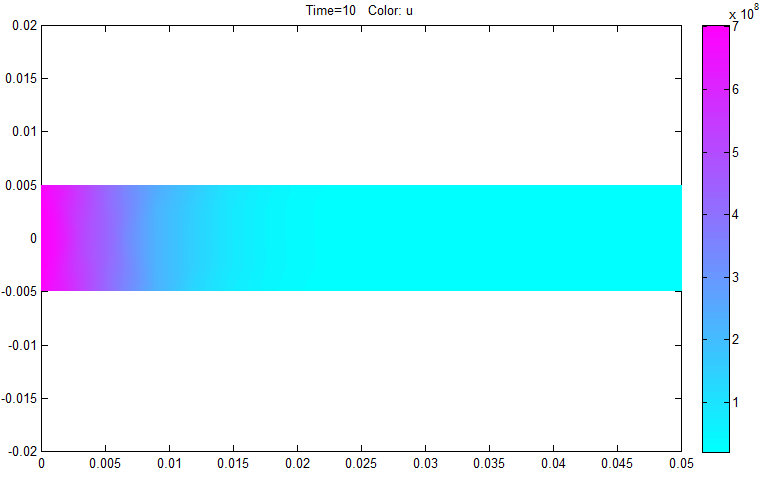
\includegraphics[scale=0.2]{./pic/04.png}}
\subfloat[$t=100$]{\centering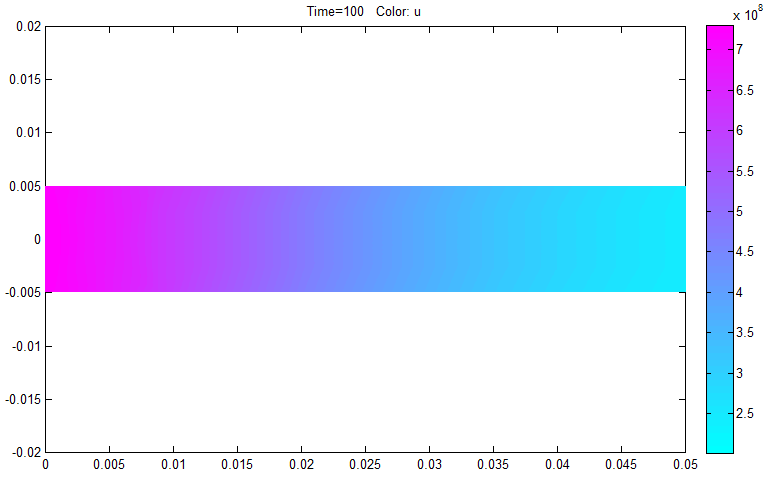
\includegraphics[scale=0.2]{./pic/04-100.png}}
\subfloat[$t=600$]{\centering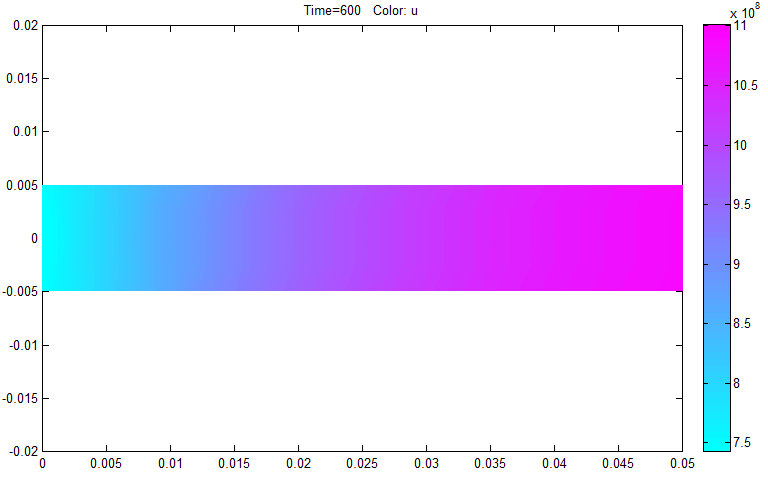
\includegraphics[scale=0.2]{./pic/04-600.png}}
%\caption{巨大芽孢杆菌的仿真结果}\label{pic:1}
\end{figure}
\end{frame}
\begin{frame}{金黄色葡萄球菌}
\begin{figure}[h]
\subfloat[$t=10$]{\centering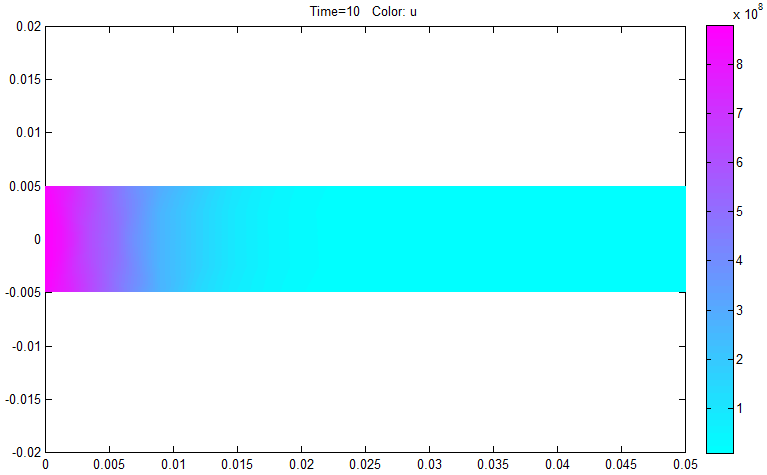
\includegraphics[scale=0.2]{./pic/05.png}}
\subfloat[$t=100$]{\centering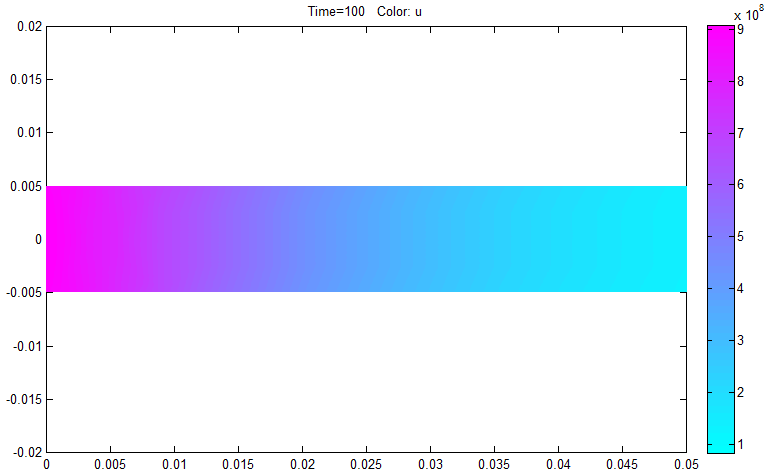
\includegraphics[scale=0.2]{./pic/05-100.png}}
\subfloat[$t=600$]{\centering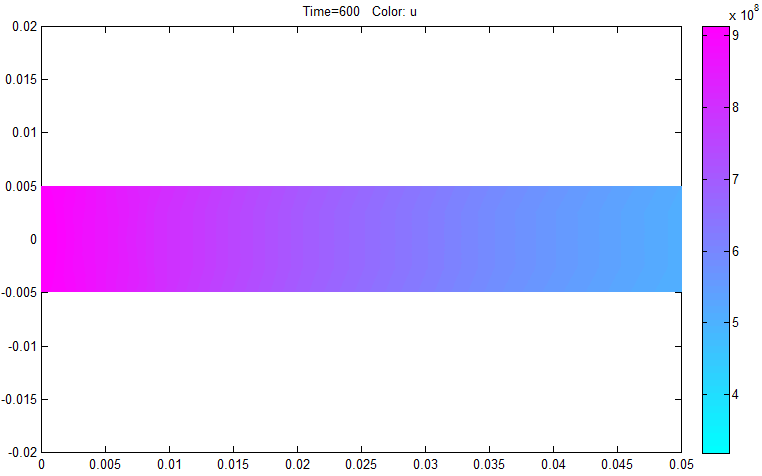
\includegraphics[scale=0.2]{./pic/05-600.png}}
%\caption{巨大芽孢杆菌的仿真结果}\label{pic:1}
\end{figure}
\end{frame}
\begin{frame}{微球菌}
\begin{figure}[h]
\subfloat[$t=10$]{\centering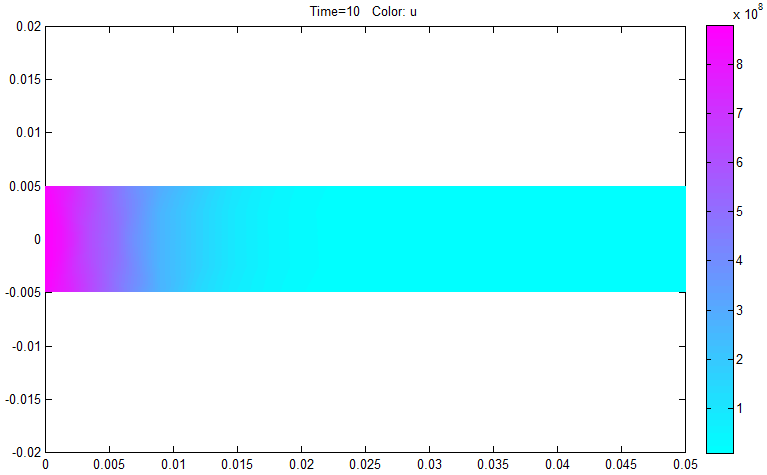
\includegraphics[scale=0.2]{./pic/05.png}}
\subfloat[$t=100$]{\centering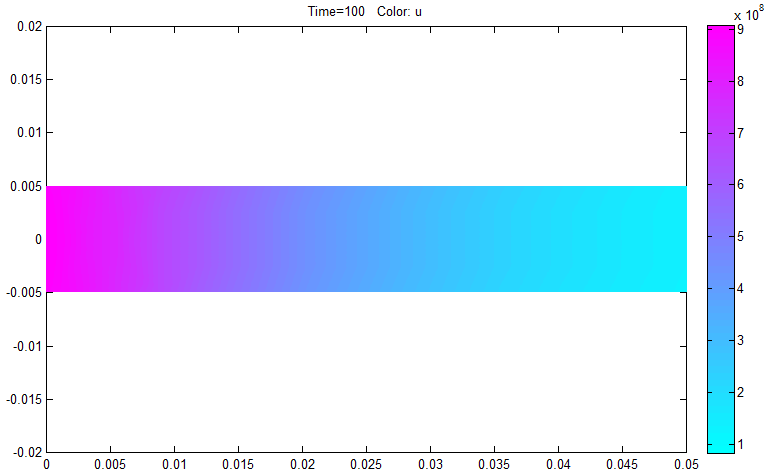
\includegraphics[scale=0.2]{./pic/05-100.png}}
\subfloat[$t=600$]{\centering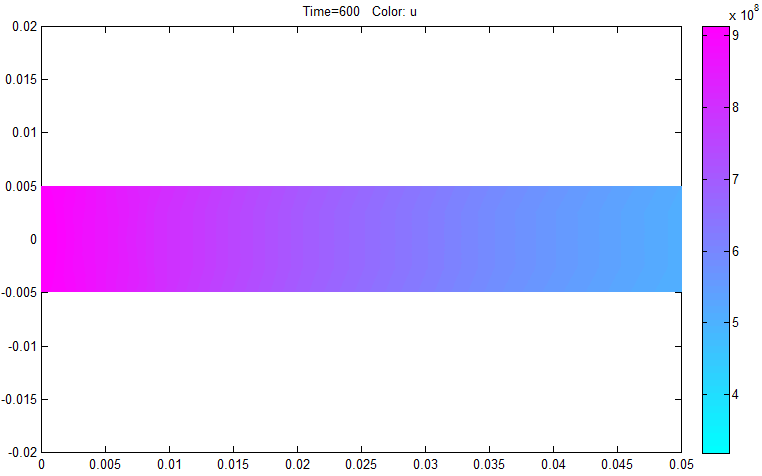
\includegraphics[scale=0.2]{./pic/05-600.png}}
%\caption{巨大芽孢杆菌的仿真结果}\label{pic:1}
\end{figure}
\end{frame}
\section{下一步的工作计划}
	\begin{frame}{需要完成的工作}
	\begin{itemize}\setlength{\itemsep}{0em}
	\fangsong
	\item 对流占优问题的差分方法
	\item 三维模型的建立与求解
	\item 仿真系统的编制
	\end{itemize}\par
	\end{frame}
	\begin{frame}{进度计划}
	\kaishu
\begin{tabularx}{10cm}{cXc}
\toprule
时间 & \centering 工作内容 & 工作地点 \\
\midrule
2013年4月					& 三维方程求解算法的研究				&	机房			  \\
2013年5月					& 数值仿真程序的编制				&	机房			  \\
2013年6月					& 完成论文						&   实验室		  \\
\bottomrule
\end{tabularx}
	\end{frame}
	\section*{}
	\begin{frame}
	\begin{center}
	\Large
	谢谢!\par
	欢迎提问
	\end{center}
	\end{frame}
\end{document}
